
%%%%%%%%%%%%%%%%%%%%%%%%%%%%%%%%%%%%%%%%%
% Arsclassica Article
% LaTeX Template
% Version 1.1 (10/6/14)
%
% This template has been downloaded from:
% http://www.LaTeXTemplates.com
%
% Original author:
% Lorenzo Pantieri (http://www.lorenzopantieri.net) with extensive modifications by:
% Vel (vel@latextemplates.com)
%
% License:
% CC BY-NC-SA 3.0 (http://creativecommons.org/licenses/by-nc-sa/3.0/)
%
%%%%%%%%%%%%%%%%%%%%%%%%%%%%%%%%%%%%%%%%%

%----------------------------------------------------------------------------------------
%	PACKAGES AND OTHER DOCUMENT CONFIGURATIONS
%----------------------------------------------------------------------------------------

\documentclass[
11pt, % Main document font size
a4paper, % Paper type, use 'letterpaper' for US Letter paper
oneside, % One page layout (no page indentation)
%twoside, % Two page layout (page indentation for binding and different headers)
headinclude,footinclude, % Extra spacing for the header and footer
BCOR5mm, % Binding correction
]{scrartcl}


 %%%%%%%%%%%%%%%%%%%%%%%%%%%%%%%%%%%%%%%%%
% Arsclassica Article
% Structure Specification File
%
% This file has been downloaded from:
% http://www.LaTeXTemplates.com
%
% Original author:
% Lorenzo Pantieri (http://www.lorenzopantieri.net) with extensive modifications by:
% Vel (vel@latextemplates.com)
%
% License:
% CC BY-NC-SA 3.0 (http://creativecommons.org/licenses/by-nc-sa/3.0/)
%
%%%%%%%%%%%%%%%%%%%%%%%%%%%%%%%%%%%%%%%%%

%----------------------------------------------------------------------------------------
%	REQUIRED PACKAGES
%----------------------------------------------------------------------------------------

\usepackage[
nochapters, % Turn off chapters since this is an article        
beramono, % Use the Bera Mono font for monospaced text (\texttt)
eulermath,% Use the Euler font for mathematics
pdfspacing, % Makes use of pdftex’ letter spacing capabilities via the microtype package
dottedtoc % Dotted lines leading to the page numbers in the table of contents
]{classicthesis} % The layout is based on the Classic Thesis style

\usepackage{arsclassica} % Modifies the Classic Thesis package

\usepackage[T1]{fontenc} % Use 8-bit encoding that has 256 glyphs

\usepackage[utf8]{inputenc} % Required for including letters with accents

\usepackage{graphicx} % Required for including images
\graphicspath{{Figures/}} % Set the default folder for images

\usepackage{enumitem} % Required for manipulating the whitespace between and within lists

\usepackage{lipsum} % Used for inserting dummy 'Lorem ipsum' text into the template

\usepackage{subfig} % Required for creating figures with multiple parts (subfigures)

\usepackage{amsmath,amssymb,amsthm} % For including math equations, theorems, symbols, etc

\usepackage{varioref} % More descriptive referencing

\usepackage{tgbonum}

\usepackage{float}
\usepackage{fontspec}
\usepackage[sfdefault]{roboto}
\usepackage[cache=false]{minted}
\usemintedstyle{borland}
\usepackage{ulem}
\usepackage{geometry}
\usepackage{lscape}





%----------------------------------------------------------------------------------------
%	THEOREM STYLES
%---------------------------------------------------------------------------------------

\theoremstyle{definition} % Define theorem styles here based on the definition style (used for definitions and examples)
\newtheorem{definition}{Definition}

\theoremstyle{plain} % Define theorem styles here based on the plain style (used for theorems, lemmas, propositions)
\newtheorem{theorem}{Theorem}

\theoremstyle{remark} % Define theorem styles here based on the remark style (used for remarks and notes)

%----------------------------------------------------------------------------------------
%	HYPERLINKS
%---------------------------------------------------------------------------------------

\hypersetup{
%draft, % Uncomment to remove all links (useful for printing in black and white)
colorlinks=true, breaklinks=true, bookmarks=true,bookmarksnumbered,
urlcolor=webbrown, linkcolor=RoyalBlue, citecolor=webgreen, % Link colors
pdftitle={}, % PDF title
pdfauthor={\textcopyright}, % PDF Author
pdfsubject={}, % PDF Subject
pdfkeywords={}, % PDF Keywords
pdfcreator={pdfLaTeX}, % PDF Creator
pdfproducer={LaTeX with hyperref and ClassicThesis} % PDF producer
}

 % Include the structure.tex file which specified the document structure and layout

\hyphenation{Fortran hy-phen-ation} % Specify custom hyphenation points in words with dashes where you would like hyphenation to occur, or alternatively, don't put any dashes in a word to stop hyphenation altogether
\fontfamily{roboto}


\ifoot{Thomas Moffat, 51337, 4042}

%----------------------------------------------------------------------------------------
%	TITLE AND AUTHOR(S)
%----------------------------------------------------------------------------------------



%----------------------------------------------------------------------------------------

\begin{document}

%----------------------------------------------------------------------------------------
%	HEADERS
%----------------------------------------------------------------------------------------

\renewcommand{\sectionmark}[1]{\markright{\spacedlowsmallcaps{#1}}} % The header for all pages (oneside) or for even pages (twoside)
%\renewcommand{\subsectionmark}[1]{\markright{\thesubsection~#1}} % Uncomment when using the twoside option - this modifies the header on odd pages
\lehead{\mbox{\llap{\small\thepage\kern1em\color{halfgray} \vline}\color{halfgray}\hspace{0.5em}\rightmark\hfil}} % The header style

\pagestyle{scrheadings} % Enable the headers specified in this block

%----------------------------------------------------------------------------------------
%	TABLE OF CONTENTS & LISTS OF FIGURES AND TABLES
%----------------------------------------------------------------------------------------

\begin{titlepage}
	\vspace{5cm}
	\centering
	{\huge\bfseries ORDR: An Sports Club kit-ordering system\par}
	\vspace{2cm}
	{\Large\itshape Thomas Moffat\par}
	\vspace{1cm}
	{Candidate Number: 4042\par}
	\vspace{1cm}
	{Centre Number: 51337}
	\vfill
\end{titlepage}

\setcounter{tocdepth}{2} % Set the depth of the table of contents to show sections and subsections only

\tableofcontents % Print the table of contents

\listoffigures



%----------------------------------------------------------------------------------------
%	ABSTRACT
%----------------------------------------------------------------------------------------


%----------------------------------------------------------------------------------------
%	AUTHOR AFFILIATIONS
%----------------------------------------------------------------------------------------



%----------------------------------------------------------------------------------------

%\newpage % Start the article content on the second page, remove this if you have a longer abstract that goes onto the second page

%----------------------------------------------------------------------------------------
%	INTRODUCTION
%----------------------------------------------------------------------------------------

\section{Analysis}
\subsection{Background to and Identification of the Problem}
The client for this program is Kira, my mother, who volunteers as a kit orders organiser for Tilehurst Swimming Club, who asked me to develop a solution for her to be able to organise kit orders more effectively. \par The current system is paper-based, so it is very slow and very inconvenient for her as it requires her to spend vast amounts of time filling in a spreadsheet in order to organise an order, and then she has to copy it all out of the spreadsheet into an email to send off to the kit suppliers. A computerised solution would alleviate some of the time required to do this and might even allow her to automate most of it.

\subsection{Interview With Primary User}
\begin{itemize}
\item What is the current system?\par

The current system is manual and uses either a paper form with a BACS (Bankers Automated Clearing Service), cheque or cash payment or an email of the same form with usually a BACS payment (sometimes a cheque delivered later) with all the relevant data being entered onto a spreadsheet for record keeping.
The data is then transferred manually to an order sheet that is used to place the order at the printers. 

The initial data required to be processed and kept track of by the club is -  Name, Number, Garment Type, Size, Personalisation, Cost, Total Cost and Payment Made.

The data required for the order sheet that is given to the printers requires only Garment Type, Size and Personalisation and is categorised by Garment Type.

\item What are the benefits of the existing system?\par
At the time of set up, this system did not require a lot of time to implement.

\item What are the drawbacks?\par
Due to its simplicity, the current system is time-consuming. Each order requires a lot of manual entry and data processing, which could easily be achieved in a more automated way. Data can get lost in between the order spreadsheet and the order sheet that is sent to the printers.

\item Which new features would be most useful?\par
\begin{itemize}

	\item A usable interface to enter the order data by the parents or by the person with the responsibility for kit ordering in the club.
	\item Storage of this data in a usable way.
	\item Automatic creation of the order sheet from the initial data on a monthly basis
	\item Emailing the order sheet to the printer with a covering email.
	\item Ability to send an email to the parents to update them with the order status.
	\end{itemize}

\item Which existing features would you like kept?\par

The new system should be based on the old system but be a better version.

\item Who would be using this system?\par
\begin{itemize}
	\item On the front end?\par
	The swimmers or swimmers’ parents or the kit order person.
	\item On the back end?\par
	The kit order person.
\end{itemize}

\item How often would you expect to be using the system?\par

The system would be used monthly to create the order sheet for the printers.

\item How often would you expect others will use the system?\par

Parents or swimmers could use the system daily to place orders.

\item Will you need any security on it?\par

Security for email addresses.
\end{itemize}

\subsection{The Current System}
The current system is paper-based, so people wanting to order kit have to download a form from the club website then fill it in and either hand it in on one a Friday night or email it to the kit email address, which then requires Kira to collate all of these orders in to one before then sending it off to the manufacturers. The kit form is seen here:
\par 
\begin{figure}[h]
	\centering
	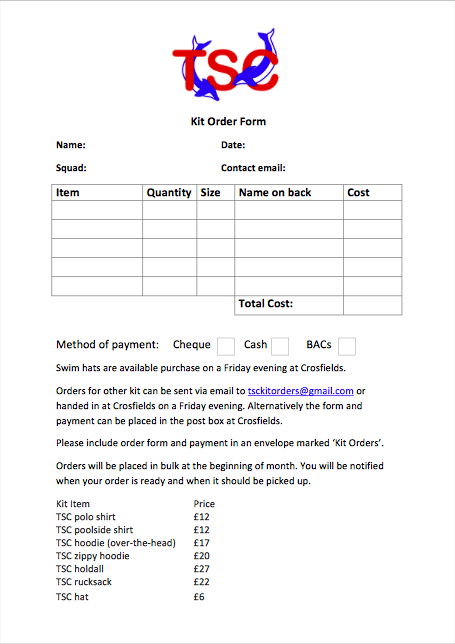
\includegraphics[scale=0.5]{TSCKitOrderForm}
	\caption{The current order form}
	\label{TSCOrderForm}
\end{figure}
\par This is obviously a very slow system, especially as the orders only get placed once a month, so it can take up to a month to receive kit that has been ordered, and possibly longer if the orders have been forgotten, which has happened far too many times in the past. This also has the problem of wasting a large amount of paper, as the forms are just collated on the computer and then discarded. \par 
Yet another problem with this system is that it requires everyone to pay attention to the dates, as missing the deadline could mean a wait of another month, and if the kit has been ordered for a large competition then it could very easily mean that the swimmers don't get what was ordered in time for the competition, as it normally takes a couple of weeks for all of the ordered kit to be printed and then picked up again. After the orders have been placed and then received, it requires Kira to email out to all the parents that their kit has been received and then requires her to bring it to a Friday-evening session when the parents are also present, and not all of the members of the squads, especially in the lowest squad swim on Fridays, so it can be a few weeks or months before the swimmers actually get the kit that was ordered. The objective for this project then, is to make a way for parents to order kit and then for Kira to be able to collate this together without hours of data entry.

\subsection{Prospective Users}
The prospective main users of this system will be Kira and then whomever takes over from her when she steps down as Kit Organiser. For this reason, I will need to assume that the users of this system are not tech-savvy, due to the fact that, while I know that Kira knows how to use computers fairly well, I don't know who will be following her so I don't know what their capabilities are regarding computers. For this reason the solution will have to be very simple so that people of any ability can use the system. \par 
The secondary users of this system will be the parents that are ordering kit using a form on the club website, so the forward-facing system will have to be very easy to use, as I don't know all of the parents so I have to assume that some of them will be tech-illiterate, or at the very least, uncomfortable with computers. 

\subsection{User Needs and Acceptable Limitations}
 Kira needs to have a way that she can have the parents order what they want and then have it in a searchable database so that she can just create an email to send to the kit manufacturers once a month. Then when she receives the kit she wants to be able to send out a mass email to the people who have ordered kit the previous month that tells them their kit is ready to be picked up. 
 \par Although the parents of the swimmers won't be the primary users, they will be affected quite a lot by the system, so it should be easy to navigate and similar in layout to the paper order form, to facilitate change-over. They will need a way to order kit, in an simple layout that then makes sure they know when their kit has been ordered and when it has come in.
 \par The acceptable limitations for this will be:\begin{itemize}
 	\item The hardware this will be running off will be somewhat underpowered, as if it is hosted locally it will be running off a 2009 MacBook Pro, and otherwise, if it is web-based it will be running on the club's web server which is not configured for a large volume of data and a large number of users using it at once.
 	\item My skills and knowledge - The system will have to not be too complex for me to create, as I have limited programming skills and limited resources. There are a few ways I could make this system, so I will have to be careful to not choose an overly simple solution, just because it is easy.
 	\item Time constraints - This system will need to be finished by February half term.
 	\item Features not able to be implemented due to complexity - Although this is an order system, it will have to work on a trust-based system as it would be far too complex for me to add in a payment solution, either involving BACS or something else. For this reason, the payments will still be processed manually, and people who haven't paid will be chased up in person. 
 	
 \end{itemize}

\subsection{Data Sources and Destinations}
The sources of data are the parents ordering kit, by way of the order form and Kira entering the details into an Excel spreadsheet. This source will not change with the new system, however it won't be via Kira, it will be automatically added in to a database. In the current system the spreadsheet is printed out and then sent off to the kit manufacturer and then Kira receives an email when they are ready for the kit to be picked up. In the new system, the data would again be arranged into a spreadsheet and printed out. This is an unfortunate limitation of the kit suppliers, not a problem on the club's end.
\begin{table}[ht]
	\small
	\caption{Current Data Sources and Destinations}
	\centering
	\makebox[\linewidth]{
	\begin{tabular}{|c|c|c|}
		\hline
		What is it & Source & Destination \\ [0.5ex]
		\hline
		Customer Details & Parents filling in an order & Excel Spreadsheet \\
		Order & Parents filling in an order & Spreadsheet \\
		Order Details & Excel Spreadsheet & Word Document\\
		\hline
		\end{tabular}}
\end{table}\par
\begin{table}[ht]
	\small
	\caption{Proposed Data Sources and Destinations}
	\centering
	\makebox[\linewidth]{
	\begin{tabular}{|c|c|c|}
		\hline
		What is it & Source & Destination \\
		\hline
		Customer Details & Parents filling in an order & customerDatabase \\
		Order details & Parents ordering kit & orderDatabase\\
		Admin Details & Kit Organiser & orderDatabase\\
		Order Details & orderDatabase & Word Document or Email\\
		\hline
		\end{tabular}}
\end{table}

\subsection{Data Volumes and Data Dictionaries}
The volume of data will be very low as the system will work entirely in text, only one person will be accessing the back-end of it, the volume of kit orders is fairly low, although high enough for this to be a problem. Also, this will only be accessed once or twice a month so the data volumes will be kept low. \par A rough calculation (using the data in Table 4) would suggest that, per order, 1156.25 bytes will be produced (i.e. 1156 bytes, 2 bits). This would suggest that, at an average order size of about 10 orders per month, the system will produce about 10kB of data per month. This is an average, there will be more produced in the run up to the large competitions of the year, and less after said competitions. 
\begin{table}[ht]
	\small
	\caption{Current Data Dictionary}
	\centering
	\makebox[\linewidth]{
	\begin{tabular}{|c|c|c|}
		\hline
		Data & Data Type & Description\\
		\hline
		Name & Text & Name of the customer\\
		Order & Text & What the customer ordered\\
		Order Quantity & Number & How many of each item was ordered\\
		Paid & Text & Shows how the customer has paid\\
		Email address & text & Customer's email address\\
		Squad & text & What swimming squad the child is in\\
		Name on back & text & what name the customer would like printed\\
		Size & text & what size the clothes are\\
		Cost & text/numbers & how much the overall cost will be\\
		\hline
		\end{tabular}}
\end{table}
\begin{table}[ht]
	\small
	\centering
	\caption{Proposed Data Dictionary}
	\makebox[\linewidth]{
	\begin{tabular}{|c|c|c|c|c|c|}
		\hline
		Field Name & Purpose & Type & Typical length (B) & Example & Validation \\ [0.5ex] % inserts table %heading
		\hline
		Name & Stores name of customer & String & 40 (320) & Alex & Not blank \\
		Ordered Kit & Stores type of kit ordered & String & 40 (320) & Polo shirt & Not blank \\
		Quantity ordered & stores number of each item & Integer & 2 (4) & 1 & >-1, <100 \\
		Paid? & Stores if order has been paid & boolean & 1 (1/8) & True & true or false \\
		Ordered & stores if order has been placed & bool & 1 (1/8) & True & true or false \\
		Email address & stores email address & String & 47 (376) & abc@abc.com & Not blank\\ 
		Name on back & stores name printed on the back & String & 10 (80) & Pedro & Not blank\\
		Squad & stores what squad swimmer is in & String & 3 (24)& Top & Not blank\\
		Size & size the items of clothing will be & String & 4 (32)& M & Not blank\\[1ex]
		\hline
		
	\end{tabular}}
	
\label{table:nonlin}
\end{table}


\subsection{Data Flow Diagrams}
\begin{figure}[H]
	\centering
	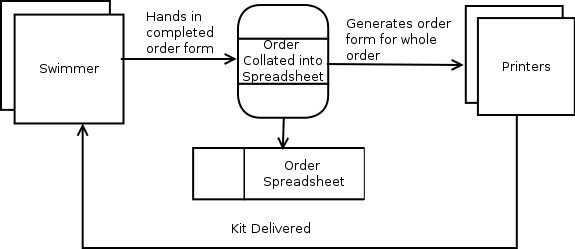
\includegraphics[width=\textwidth]{CurrentLvl0}
	\caption{A level 0 data flow diagram of the current system}
	\label{CurrentLvl0}
\end{figure}
\begin{figure}[H]
	\centering
	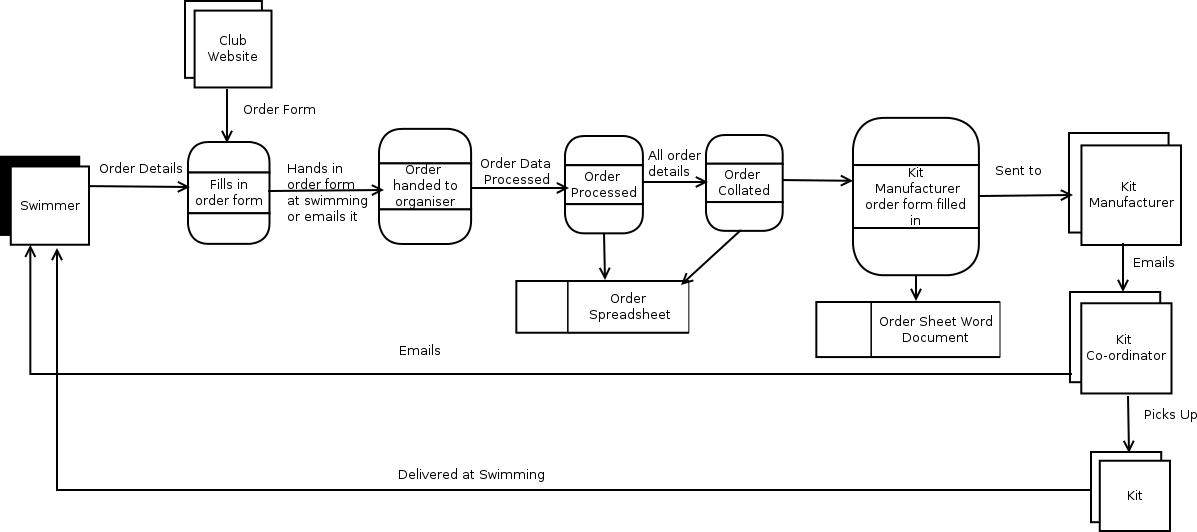
\includegraphics[scale = 0.35]{CurrentLvl1}
	\caption{A level 1 data flow diagram of the current system}
	\label{CurrentLvl1}
\end{figure}
\begin{figure}[H]
	\centering
	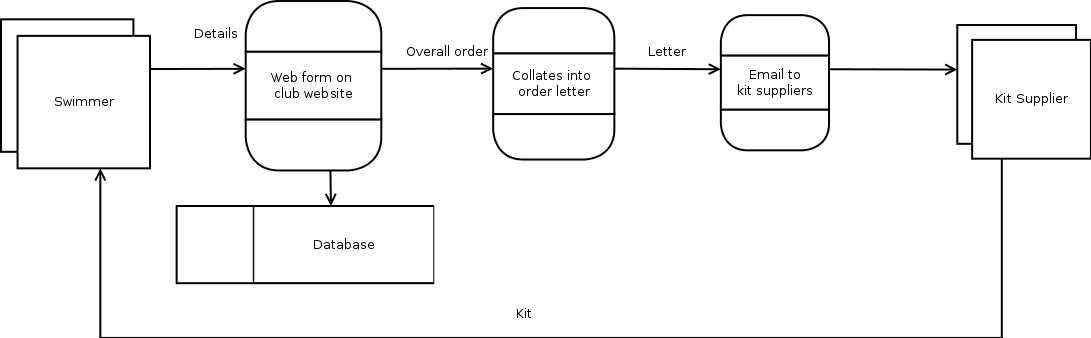
\includegraphics[width=\textwidth]{ProposedLvl0}
	\caption{A level 0 data flow diagram of the proposed system}
	\label{ProposedLvl0}
\end{figure}
\begin{figure}[H]
	\centering
	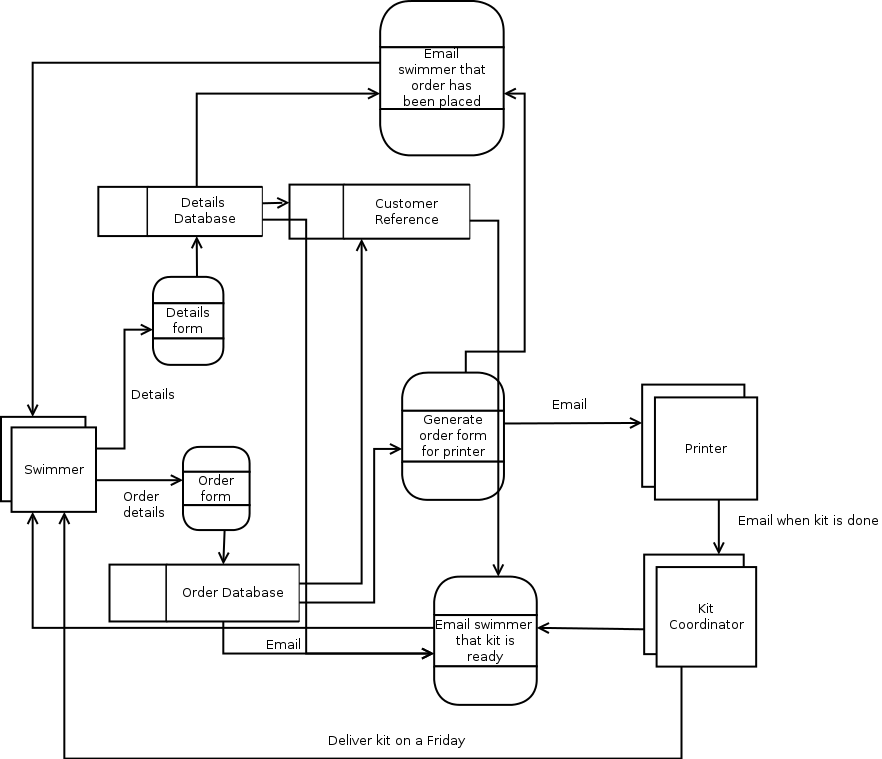
\includegraphics[width=\textwidth]{ProposedLvl1}
	\caption{A level 1 data flow diagram of the proposed system}
	\label{ProposedLvl1}
\end{figure}
The proposed system as seen in figure \ref{ProposedLvl1} is rather more complicated than the current system seen in figure \ref{CurrentLvl1} which unfortunately means that there are more things that will need to be kept track of and so more things that could potentially break, however this will be traded off with a massive increase in convenience for everyone, not to mention that most of the system can be automated which will reduce the kit coordinator's workload. This will also mean that the system will be much faster, as orders will be entered into the system immediately and so will not be forgotten, unlike in the current system.

\subsection{Entity Relationship Models}

\begin{figure}[H]
	\centering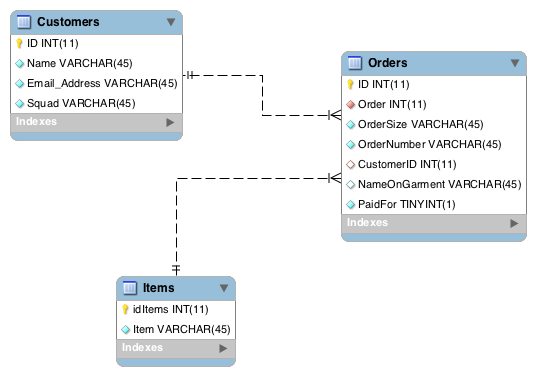
\includegraphics[width=\textwidth]{EERProp}
	\caption{The proposed Entity Relationship diagram, exported from MySQLWorkbench}
	\label{PropEER}	
\end{figure}
As can be seen in figure \ref{PropEER}, the proposed EER will be fairly simple, with some foreign keys.

\subsection{Entity Description}

Customer(\uline{ID}, Name, Email\_Address, Squad)\\
Order(\uline{ID}, Order (Foreign key from Items), OrderSize, OrderNumber, CustomerID (Foreign key from Customer), NameOnGarment)\\
Items(\uline{idItems}, Item)

\subsection{Objectives for the Proposed System}
The objectives of this system are to have an easy to use system that will run on minimal hardware. More specifically  \begin{enumerate}
	\item It must have a well-structured (1NF or 2NF) database system that can be easily accessed.
	\item It must have some sort of user interface allowing a person to enter the data then have the program handle the sorting.
	\item It must store the data in a usable way (Most likely plain text).
	\item It must have a search function, so the kit coordinator can search the database for certain attributes, like, for example, people who have and haven't paid for their order.
	\item It must be lightweight enough to be run on a web server, such as the one hosting the club website.
	\item It should have a way to automate the kit ordering procedure, by generating the order form that is sent off to the kit printers.
	\item It should have a web-based front end so the orders for kit can be placed via the club website.
	\item It should be able to send a mass email to all of the people who have ordered kit.
	\item It could have an ability to monitor the email inbox of the kit email address so when the printer emails that the kit is ready it will send out a mass email automatically to everyone that has ordered.
	\item It would be nice to have an integrated payments solution so everything could be done through the web interface, although due to time and complexity constraints this probably won't happen.
\end{enumerate}

\subsection{Potential Solutions}
The potential solutions for this project are:\begin{itemize}
	\item An Excel spreadsheet using a VBA front-end application
	\item A VB.NET front-end application and a Microsoft Access database on the back-end
	\item A fully bespoke system programmed in Java and HTML
	\item A fully bespoke system programmed in C++
\end{itemize}
The respective advantages and disadvantages are seen in the next section.

\subsection{Feasibility of Potential Solutions}
\begin{itemize}
	\item An Excel spreadsheet using a VBA front-end. Advantages:\begin{itemize}
		\item It would be exceedingly easy to implement, as it just requires a spreadsheet and a small amount of programming to get up and running.
		\item User already has experience using Excel and so would be able to use the system with minimal help.
	\end{itemize}
	Disadvantages:\begin{itemize}
		\item This solution would be offline only, so one of the main features of the proposed solutions, the online ordering system, would have to be left out, or radically changed.
		\item Excel is a flat file database, which doesn't lead to good database design practices and also won't let me handle links between data.
		\item The current system involves Excel so the new system would be too similar to the current system, and so wouldn't follow what the client wanted. 
	\end{itemize}
	\item A VB.NET front-end application and a Microsoft Access database back-end. Advantages:\begin{itemize}
		\item Most of the system is pre-implemented so it would require a minimal amount of work to get up and running.
		\item Unlike the Excel spreadsheet, data can be linked to and the database won't be just flat.
	\end{itemize}
	Disadvantages:\begin{itemize}
		\item I have no experience using VB.NET, which would add an unnecessary level of complexity to the project, as I would need to learn VB.NET as I worked.
		\item I don't have convenient access to a copy of Microsoft Access, which would mean that I would need to purchase a copy.
		\item The solution will be offline only, which will mean that orders wouldn't be able to be placed through the website.
		\end{itemize}
	\item A bespoke coded system in Java. Advantages:\begin{itemize}
		\item It would allow me to control and integrate everything from the beginning, as I would be creating most of the system from scratch.
		\item There would be no outlay, as I can use a free IDE to develop in, and Java which is itself free.
		\item The system won't be a flat file database, so I will be able to have links between data.
		\item Thanks to JDBC, the database will be searchable using SQL statements.
		\item The solution will be able to be hosted online and allow the kit coordinator to log in to the back end to view the database.
	\end{itemize}
	Disadvantages:\begin{itemize}
		\item Java can be unnecessarily complex to write a program in.
		\item Java can be a massive resource hog, which means that it would be tricky to run on a low-budget web server.
		\item I have minimal experience programming in HTML.
	\end{itemize}
	\item A bespoke coded solution in C++. Advantages:\begin{itemize}
		\item C++ is a fairly low-level language, so it's quite powerful
		\item It has a large community, so if I get stuck with a problem then I can research solutions with little time wasted.
	\end{itemize}
	Disadvantages:\begin{itemize}
		\item I have absolutely no knowledge of programming using C++ so I would have to spend a lot of time learning how to code using it, which could be better spent programming the solution. 
		\item Is apparently not very good for cross-platform applications, as a library is normally chosen which is platform specific, although due to my lack of knowledge of this language I don't know if this is true or not.
	\end{itemize}
\end{itemize}

\subsection{Justification of Chosen Solution}
I will be making a bespoke solution in Java for this project, as I have far more experience in this language than any of the other solutions that I proposed. I also feel this will be the best as Java is incredibly versatile, and so can be run on any platform with minimal amounts of set-up. It does not require any purchase to be made, unlike Microsoft products which means that it can be made on a shoestring budget. \par Also due to Java's ubiquity it has a vast number of resources that will be very helpful for referring to, if I get stuck with a certain section of this project. It has very good integration with SQL thanks to JDBC, which will mean that everything can be integrated into one complete package, rather than relying on solutions that could break if there is an update to the commercial software package being used. This integration will also mean that I will be able to make the database searchable via SQL queries, which will definitely improve workflow as the kit organiser will be able to search for, for instance, people who haven't paid. \par Although Java is normally seen as quite a resource intensive language, I think that, if the program stays small it will be relatively lightweight to run on the server. I will be able to deal with the relative complexity of Java as a language by ensuring that my design is logical and methodical. \par While I do have minimal experience using HTML, I feel that this will be the easiest way to create a web form, as opposed to coding an applet in Java. This is due to the fact that I experimented with making a JApplet and decided that it was too convoluted for what I wanted to do and would have bogged me down, trying to get it to work. 




\section{Design}

\subsection{Overall System Design}
\begin{table}[H]
\small
\centering
\caption{Summary Table}
\makebox[\linewidth]{
\begin{tabular}{|c|c|}
	\hline
	Inputs & Processes \\ [0.5ex]
	\hline
	Swimmer's name & Add new Order\\
	Email Address & Add new customer\\
	Squad & Compile order to send off\\
	Name on Garments & Edit order\\
	Order & Show all orders to Kit Co-ordinator\\
	Size of the Garment & \\
	Number of Garments ordered & \\
	Whether the order has been paid for & \\
	\hline
	Tables Storing Data & Outputs\\ [0.5ex]
	\hline
	Order Details & Compiled Order Form \\
	Customer Details & Certain Orders via Search Function \\
	Items Available & All orders in table to kit co-ordinator\\
	\hline
	
	
\end{tabular}}
\end{table}

\subsection{Description of Modular System Structure}
\begin{figure}[H]
\centering
\includegraphics[scale=0.5]{customer}
\caption{The part of the project facing the customer. This is all written in web-based technology}
\label{Customer}
\end{figure}
\begin{figure}[H]
\centering
\includegraphics[scale=0.5]{KitCoordinator}
\caption{The part of the project facing the Kit Coordinator. This is all written in Java, except for the SQL script and the CSV}
\label{KitCoordinator}	
\end{figure}

\begin{table}[H]
\tiny
\centering
\makebox[\linewidth]{
\begin{tabular}{|c|c|c|c|c|c|c|c|c|c|}
\hline
Ordr &  &  &  &  &  &  &  &  &  \\ 
\hline
MainMenu &  &  & Get Connection &  &  & Remake Database &  &  & \\ 
\hline
Display & Enter Sort & Enter Search String & Open XML File & Get Connection Details & Return & Open SQL File & Run Script & Open CSV & Execute\\ 
\hline \\ 
\hline\end{tabular}}
\label{table:table}
\caption{\small{}} 
\end{table}
\begin{table}[H]
\tiny
\centering
\makebox[\linewidth]{
\begin{tabular}	
\end{table}





\subsection{Design Data Dictionary}

\subsection{Database Design}

\subsection{Identification of Storage Material and Format}

\subsection{Identification of Processes and Algorithms for Data Transformation}

\subsection{User Interface Design and Rationale}

\subsection{Planned Data Capture and Entry}

\subsection{Planned Valid Output Designs}

\subsection{Measures Planned for Security and Integrity of Data}
To make sure the data input is valid, the program will make sure that the data entered has the expected hallmarks of the entered data. So, for instance, if an email address is entered, the program will check to see if the string has an @ symbol in it (done via HTML form and specifically the email field within it), and it will make sure that there is a domain name, although due to the manual element of the program, where everything is checked by eye before it is sent off, whether the domain is valid or not won't matter. The back-up strategy will involve a back-up whenever the website of the swimming club is backed up. This will ensure that the database backup is always as up to date as the website itself is.

\subsection{Measures Planned for System Security}
The database will be password protected, and this will be entered when someone attempts to connect to it. I am planning to do this using SSL, however I am not sure what this will be like to implement so it may have to be scaled back somewhat or possibly abandoned, depending on the complexity and whether I can obtain a signed certificate, which should be possible using Let'sEncrypt. No matter what happens the password will never be sent via plaintext, it will be salted and hashed on the client machine then sent to the server. To prevent SQL Injections, I will be making all of the SQL queries that the user can influence (for instance, the search query) Prepared Statements, which escape any special characters, hence foiling their dastardly plots to ruin my database. 

\subsection{Overall Test Strategy}
To begin with I will be performing black box testing. In this stage of the testing I will be creating fake orders and seeing what happens when they are fed into the system. The expected output should be exactly the same as what is input, unless what is input is too long for the SQL field, or the input is invalid (for instance trying to input a SQL command into the text-boxes and so trying to perform a SQL injection. This should be prevented due to the use of prepared statements but I will test these just to make sure). For the web based part of this project this will involve testing in Google Chrome and Safari to see if the CSS works and it passes to the database correctly in both browsers.\par This will be followed by white box testing where I will test every part of the system individually, and make sure I get the outputs that I expect. To achieve this I will insert print statements in parts of my code and then trigger the classes that they are in in order to trace their progress through the execution of the program. 





\section{Technical Solution}

\section{Source Code Appendix}
\newgeometry{left=1cm, right=1cm}
\inputminted[linenos, breaklines]{java}{/Users/tsmoffat/kitordersystem/kitordersystem/kitordersystem/MainMenu.java}
\inputminted[linenos, breaklines]{java}{/Users/tsmoffat/kitordersystem/kitordersystem/kitordersystem/getConnection.java}
\inputminted[linenos, breaklines]{java}{/Users/tsmoffat/kitordersystem/kitordersystem/kitordersystem/TableViewTest.java}
\inputminted[linenos, breaklines]{java}{/Users/tsmoffat/kitordersystem/kitordersystem/kitordersystem/DocWriter.java}
\inputminted[linenos, breaklines]{java}{/Users/tsmoffat/kitordersystem/kitordersystem/kitordersystem/DBSearch.java}
\inputminted[linenos, breaklines]{java}{/Users/tsmoffat/kitordersystem/kitordersystem/kitordersystem/CSVReader.java}
\inputminted[linenos, breaklines]{java}{/Users/tsmoffat/kitordersystem/kitordersystem/kitordersystem/DBReset.java}
\inputminted[linenos, breaklines]{SQL}{/Users/tsmoffat/kitordersystem/kitordersystem/kitordersystem/KitOrderProper.sql}
\inputminted[linenos, breaklines]{html}{/Users/tsmoffat/kitordersystem/kitordersystem/kitordersystem/WebInput.html}
\inputminted[linenos, breaklines]{html}{/Users/tsmoffat/kitordersystem/kitordersystem/kitordersystem/WebInputOrder.html}
\inputminted[linenos, breaklines]{CSS}{/Users/tsmoffat/kitordersystem/kitordersystem/kitordersystem/styling.css}
\inputminted[linenos, breaklines]{php}{/Users/tsmoffat/kitordersystem/kitordersystem/kitordersystem/dbcustomerupdate.php}
\inputminted[linenos, breaklines]{php}{/Users/tsmoffat/kitordersystem/kitordersystem/kitordersystem/DBOrderUpdate.php}
\restoregeometry





%----------------------------------------------------------------------------------------
%	BIBLIOGRAPHY
%----------------------------------------------------------------------------------------

\renewcommand{\refname}{\spacedlowsmallcaps{References}} % For modifying the bibliography heading

\bibliographystyle{unsrt}

\bibliography{sample.bib} % The file containing the bibliography

%----------------------------------------------------------------------------------------

\end{document}